\chapter{Train Benchmark Technical Specifications}

\todo{write about original, extended overview}

\section{Original Version}

A \concept{test case} configuration for every tool consists of an \emph{instance model} (\secref{sec:instanceGeneration}) with a \emph{given size} to be checked, a \emph{predefined query} (\secref{sec:queries}) describing constraint voilating elements, and the name of the \emph{scenario} (\secref{sec:scenarios}) to be run.

As a result of a run testcase, the \emph{execution times} of the phases, \emph{memory usage}, and the \emph{number of erroneous elements} are measured. The number of invalid elements are used to check the correctness of the validation, however elements must be available for later processing. 


\subsection{Phases}
\label{sec:phases}

\begin{figure}[Htb]
	\centering
	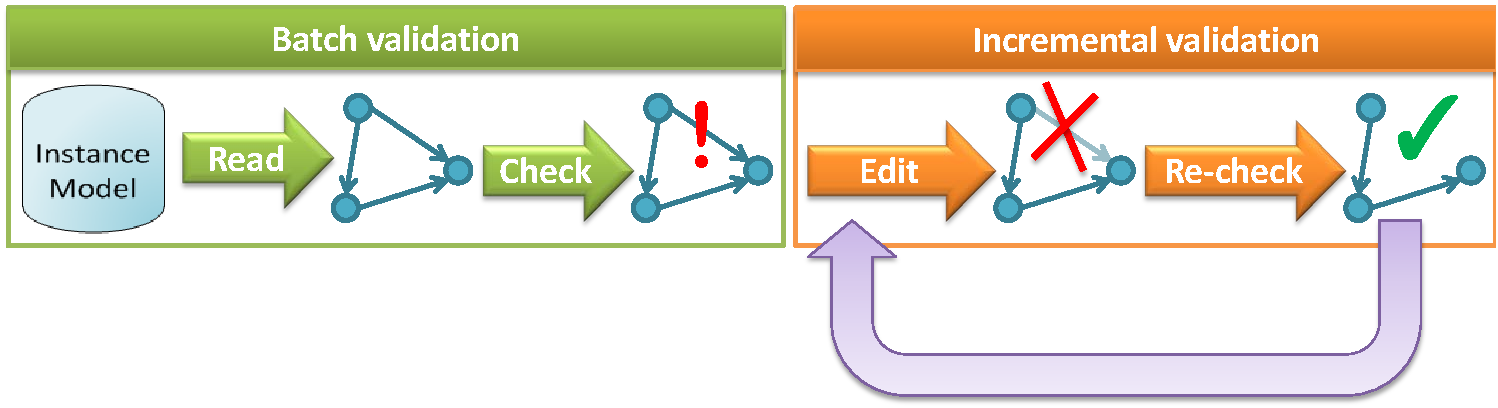
\includegraphics[scale=0.5]{figures/phases}
	\caption{Four phases of the benchmark}
	\label{fig:phases}
\end{figure}

To measure performance also when the underlying model is changing, four benchmark \concept{phases} were defined, as illustrated in \figref{fig:phases}.
\begin{enumerate}
 
 \item During the \concept{read} phase, the previously generated instance model and validation query are loaded from hard drive to memory. This includes the parsing of the input as well as initializing data structures of the tool.
 
 \item In the \concept{check} phase, the instance model is queried to identify invalid elements. This can be as simple as reading the results from cache, or the model can be traversed based on some index. By the end of this phase, erroneous objects need to made available in a list for further processing.
 
 \item In the \concept{edit} phase, the model is changed to simulate effects (and measure performance) of model modifying operations. At the beginning of this phase ``query like'' functions are used to gather elements to be modified, however this time is excluded, and only the required time of model editing operations are recorded in this phase. (As query performance is measured in the check phases.)
 
 \item The re-validation of the model is carried out in the \concept{re-check} phase similarly to the \emph{check} phase.
\end{enumerate}

\subsection{Use-case scenarios of the benchmark}
\label{sec:scenarios}

\todo{lehet a köv. bekezdést át kellene fogalmazni.}
Paper \cite{icgt08-bhrv} analyzes performance of algorithms used for graph
pattern query answering, and identifies two use-cases where efficient
\emph{incremental model validation} is required. The batch part of our benchmark
consists of the execution of the read and first check phases. Inspired by paper
\cite{icgt08-bhrv}, three \concept{scenarios} were defined to measure different
use-cases:
\begin{itemize}
  
  \item \concept{Batch validation scenario:}
  In this scenario the model is \emph{read} in one batch from storage, than a model validation is carried out by executing the query in the check phase. Such use-case is performed when a model editor is opened, and initial validations are issued by the designer. 
  
  \item \concept{Model transformation scenario:}
  The automated model transformation scenario extends the batch validation scenario by differential model modification and re-checking phases. In the edit phase, the model is corrected, based on the erroneous objects identified during the batch validation. This is carried out by the tool itself performing mass edits automatically. Finally, the whole model is re-checked, and remaining or newly introduced errors are reported. 
  
  Efficient execution of such a use-case is necessary during refactoring, incremental code generation, or when a model is transformed from a source language to a target language by a model transformation program, using model synchronisation.
  
  \item \concept{User model editing scenario:}
  The user model editing scenario extends the batch validation scenario by differential model modification and re-checking phases. After the batch validation a small model manipulation step is performed (e.g. a reference is deleted), which is immediately followed by re-validation to get instantaneous feedback.  In this scenario such small edit and re-check phases are executed in sequence.
  
  Such scenario occurs when someone uses a common UML editor (for designing software solutions), or a domain-specific editor where elements or relations are added one-by-one. These editors should detect quickly design errors early in the development process to let engineers refine models and cut down debugging and error correction costs.
  
\end{itemize}


\subsection{Metamodel}
\label{sec:domain}

\begin{figure}[htb!]
\begin{center}
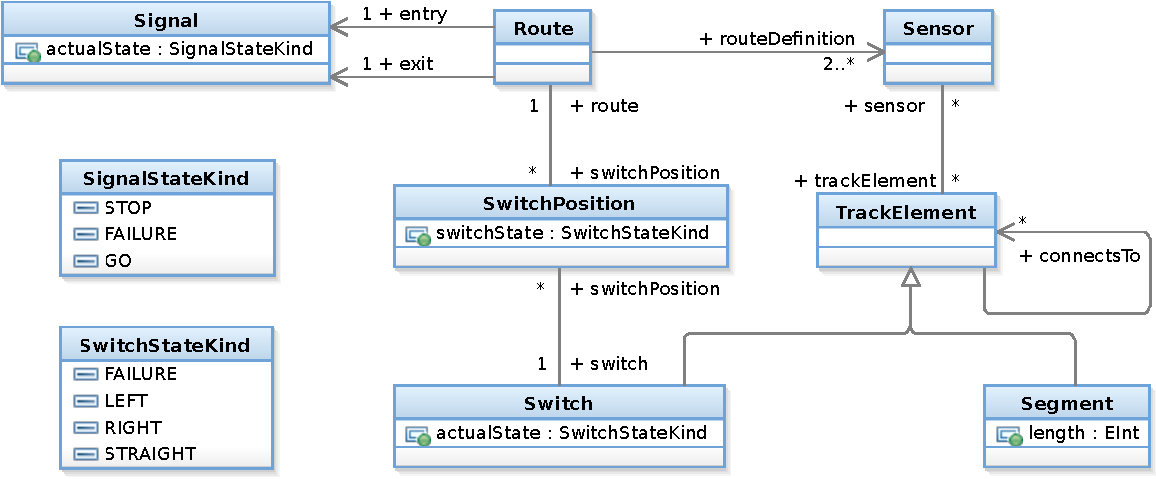
\includegraphics[width=1\columnwidth]{figures/TrainMM.pdf}
\caption{Train Metamodel}
\label{fig:metamodel}
\end{center}
\end{figure}


Throughout the paper, an example from the railway domain is used which is depicted on \figref{fig:metamodel}. A train \emph{route} can be defined by a set of \emph{sensors}. Sensors are associated with \emph{track elements}, which can be a track \emph{segment} (with length) or a \emph{switch}. A route can have associated \emph{switch positions}, which describe the required state of a switch belonging to the route. Different route definitions can specify different states for a specific switch.
 
\subsection{Queries}
\label{sec:queries}

In the validation and re-validation phase of the benchmark, constraint violating elements are returned by queries. These constraints are first defined informally in plain text and then formalized using a query language suited for the benchmarked tool. As a result, the query must return invalid instance model elements.
 
Two simple queries involving maximum two objects (named PosLength and SwitchSensor) and two complex queries involving 4-7 variables and joins (called RouteSensor and SignalNeighbor) were defined. Simple queries can filter less efficient tools, and complex queries can be used to differentiate faster model query technologies.
 
In the following, we present the queries defined in the \tb{}. We describe the semantics and the goal of each query. We also show the associated graph pattern and relational algebra query.

\todo{meggondolandó, hogy a TP-ben ``Virtuoso szerű leképezésről'' (relációs dolgokról) itt beszéljünk-e}

\subsubsection{Relational Schemas}

For formulating the queries in relational algebra we define the following relational schemas for representing the vertices (objects) in the graph (instance model).

\begin{itemize}
  \item $ \mathit{Route}\left(\mathit{id}\right) $
  \item $ \mathit{Sensor}\left(\mathit{id}, \mathit{Segment\_length}\right) $
  \item $ \mathit{Signal}\left(\mathit{id}\right) $
  \item $ \mathit{Switch}\left(\mathit{id}\right) $
  \item $ \mathit{SwitchPosition}\left(\mathit{id}\right) $
  \item $ \mathit{TrackElement}\left(\mathit{id}\right) $
\end{itemize}

The edges (relationships) are represented with the following relational schemas:

\begin{itemize}
  \item $ \mathit{Route\_entry}\left(\mathit{Route}, \mathit{Signal}\right) $
  \item $ \mathit{Route\_exit}\left(\mathit{Route}, \mathit{Signal}\right) $
  \item $ \mathit{Route\_switchPosition}\left(\mathit{Route}, \mathit{SwitchPosition}\right) $
  \item $ \mathit{Route\_routeDefinition}\left(\mathit{Route}, \mathit{Sensor}\right) $
  \item $ \mathit{SwitchPosition\_switch}\left(\mathit{SwitchPosition}, \mathit{Switch}\right) $
  \item $ \mathit{TrackElement\_sensor}\left(\mathit{Switch}, \mathit{Sensor}\right) $
  \item $ \mathit{TrackElement\_connectsTo}\left(\mathit{TrackElement}, \mathit{TrackElement}\right) $
\end{itemize}

\subsubsection{Graph Patterns}

Blue rectangles and arrows mark simple constraints, while red rectangles and arrows represent negative application conditions. The query return with the nodes in hollow blue rectangles. Additional constraints (e.g.\ arithmetic comparisons) are shown in the figure in text.

%%%%%%%%%%%%%%%%%%%%%%%%%%%%%%%%%%%%%%%%%%%%%%%%%%%%%%%%%%%%%%%%%%%%%%%%%%%%%%%
\subsubsection{Query: PosLength}

\paragraph{Description.} The \textit{PosLength} well-formedness constraint requires that a segment must have positive length. Therefore, the query (\figref{fig:trainbenchmark-poslength}) checks for segments with a length less than or equal to zero. The SPARQL representation of the query is shown in \lstref{lst:poslength-sparql}.

\paragraph{Goal.} The query checks whether an object has an attribute. If it does, the value is checked. Checking attributes is a real world use case, even if a very simple one. Note that simple string checking is also measured in the Berlin SPARQL Benchmark \cite{BSBM}, and it concludes that the string comparison algorithm dominates the query time.

\begin{figure}[Htb]
\centering
\begin{minipage}{0.5\textwidth}
  { \alignListing
    \sourceSPARQL{figures/queries/PosLength.sparql}}
  \caption{PosLength query in SPARQL}
  \label{lst:poslength-sparql}
\end{minipage}
\end{figure}

% 
% \lstset{language=SQL,morekeywords={PREFIX,FILTER,OPTIONAL,BOUND}}
% 
% \begin{lstlisting}[caption=The PosLength query in SPARQL, label=lst:poslength-sparql]
% PREFIX base: <http://www.semanticweb.org/ontologies/2011/1/TrainRequirementOntology.owl#>
% PREFIX rdfs: <http://www.w3.org/2000/01/rdf-schema#>
% PREFIX owl:  <http://www.w3.org/2002/07/owl#>
% PREFIX rdf:  <http://www.w3.org/1999/02/22-rdf-syntax-ns#>
% 
% SELECT DISTINCT ?xSegment
% WHERE
% {
%     ?xSegment rdf:type base:Segment .
%     ?xSegment base:Segment_length ?xSegment_length .
% 
%     FILTER (?xSegment_length <= 0)
% }
% \end{lstlisting}

\begin{figure}[Htb]
		\centering
		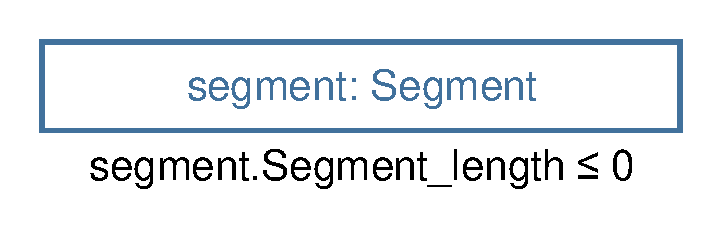
\includegraphics[scale=0.4]{figures/trainbenchmark-poslength}
		\caption{The PosLength query's pattern}
		\label{fig:trainbenchmark-poslength}
\end{figure}

\paragraph{Relational algebraic form.} The \textit{PosLength} query can be formalized in relational algebra as:

$$ \pi_{\mathit{Sensor\_id}} \left( \sigma_{\mathit{Segment\_length} \leq 0} \left( \mathit{Sensor} \right) \right) $$

%%%%%%%%%%%%%%%%%%%%%%%%%%%%%%%%%%%%%%%%%%%%%%%%%%%%%%%%%%%%%%%%%%%%%%%%%%%%%%%
\subsubsection{RouteSensor}

\paragraph{Description.} The \textit{RouteSensor} well-formedness constraint requires that all sensors that are associated with a switch that belongs to a route must also be associated directly with the same route. Therefore, the query (\figref{fig:trainbenchmark-routesensor}) looks for sensors that are connected to a switch, but the sensor and the switch are not connected to the same route. The SPARQL representation of the query is shown in \lstref{lst:routesensor-sparql-nac}.

\paragraph{Goal.} This pattern checks for the absence of circles, so the efficiency of the join and the antijoin operations is tested.

\begin{figure}[Htb]
\centering
\begin{minipage}{0.5\textwidth}
  { \alignListing
    \sourceSPARQL{figures/queries/RouteSensor_neg.sparql}}
  \caption{RouteSensor query in SPARQL}
  \label{lst:routesensor-sparql-nac}
\end{minipage}
\end{figure}

\paragraph{Remark.} Note that the negative application condition (NAC) part (\texttt{FILTER NOT EXISTS}) is a SPARQL 1.1 feature. In SPARQL 1.0, we have to use the approach shown in \lstref{lst:routesensor-sparql-nac10}.

\begin{figure}[Htb]
\centering
\begin{minipage}{0.5\textwidth}
  { \alignListing
    \sourceSPARQL{figures/queries/RouteSensor.sparql}}
  \caption{RouteSensor query in SPARQL 1.0}
  \label{lst:routesensor-sparql-nac10}
\end{minipage}
\end{figure}

% \begin{lstlisting}[caption=The RouteSensor query in SPARQL, label=lst:routesensor-sparql]
% PREFIX base: <http://www.semanticweb.org/ontologies/2011/1/TrainRequirementOntology.owl#>
% PREFIX rdfs: <http://www.w3.org/2000/01/rdf-schema#>
% PREFIX owl:  <http://www.w3.org/2002/07/owl#>
% PREFIX rdf:  <http://www.w3.org/1999/02/22-rdf-syntax-ns#>
% 
% SELECT DISTINCT ?xSensor
% WHERE
% {
%     ?xRoute rdf:type base:Route .
%     ?xSwitchPosition rdf:type base:SwitchPosition .
%     ?xSwitch rdf:type base:Switch .
%     ?xSensor rdf:type base:Sensor .
%     ?xRoute base:Route_switchPosition ?xSwitchPosition .
%     ?xSwitchPosition base:SwitchPosition_switch ?xSwitch .
%     ?xSwitch base:TrackElement_sensor ?xSensor .
% 
%     FILTER NOT EXISTS {
%         ?xRoute ?Route_routeDefinition ?xSensor .
%     } .
% }
% \end{lstlisting}
% 
% \begin{lstlisting}[caption=SPARQL 1.0 formula for the NAC part of the RouteSensor query, label=lst:routesensor-sparql-nac]
%     OPTIONAL {
%         ?xRoute ?Route_routeDefinition ?xSensor .
%         FILTER (sameTerm(base:Route_routeDefinition, ?Route_routeDefinition))
%     } .
%     FILTER (!bound(?Route_routeDefinition))
% \end{lstlisting}

\begin{figure}[Htb]
		\centering
		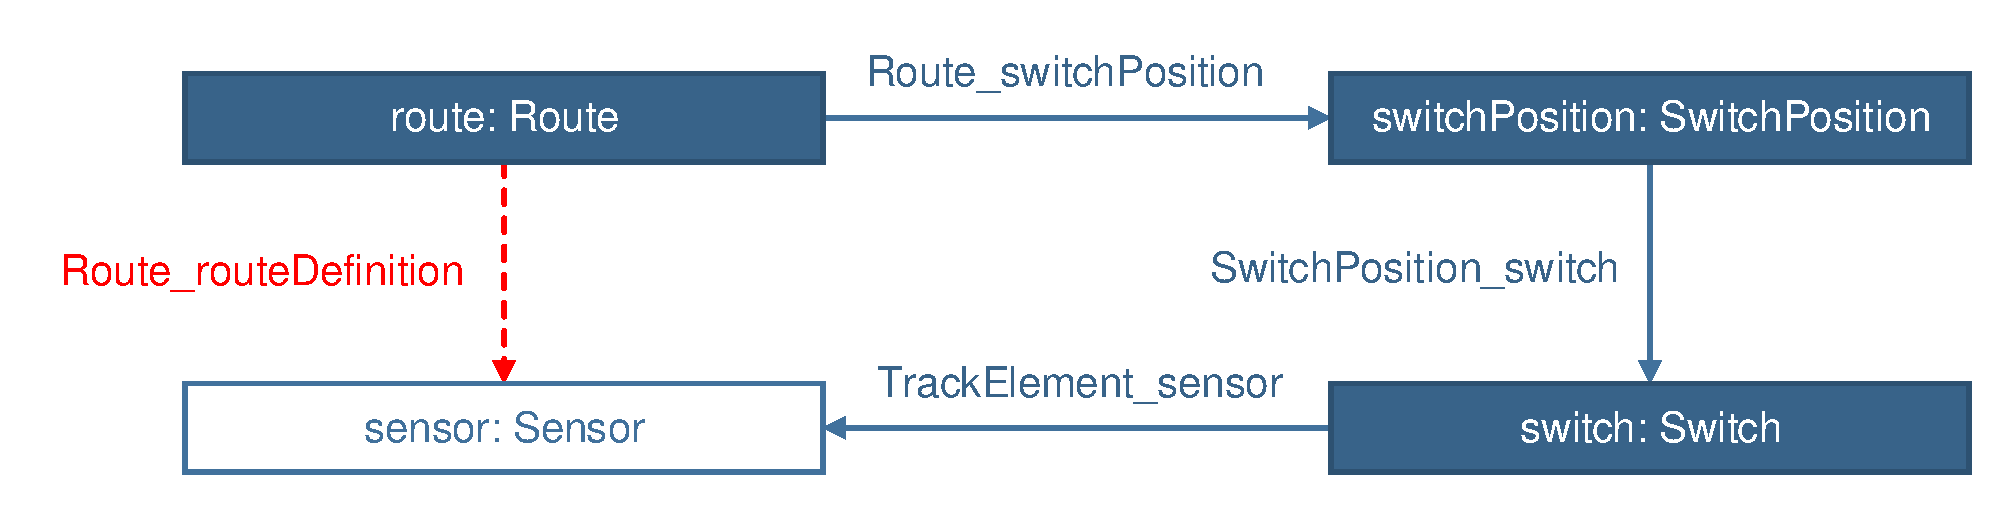
\includegraphics[scale=0.4]{figures/trainbenchmark-routesensor}
		\caption{The RouteSensor query's pattern}
		\label{fig:trainbenchmark-routesensor}
\end{figure}

\paragraph{Relational algebraic form.}  The \textit{RouteSensor} query can be formalized in relational algebra as:

\begin{align*}
& \pi_{\mathit{Route}} \big( \\
& \quad \mathit{Route\_switchPosition} \naturaljoin \mathit{SwitchPosition\_switch} \naturaljoin \\
& \quad \mathit{TrackElement\_sensor} \antijoin \mathit{Route\_routeDefinition} \\
& \big)
\end{align*}

%%%%%%%%%%%%%%%%%%%%%%%%%%%%%%%%%%%%%%%%%%%%%%%%%%%%%%%%%%%%%%%%%%%%%%%%%%%%%%%
\subsubsection{SignalNeighbor}

\paragraph{Description.} The \textit{SignalNeighbor} well-formedness constraint requires that routes that are connected through sensors and track elements have to belong to the same signal. Therefore, the query (\figref{fig:trainbenchmark-signalneighbor}) checks for routes which have an exit signal and a sensor connected to another sensor (which is in a definition of another route) by two track elements, but there is no other route that connects the same signal and the other sensor. The SPARQL representation of the query is shown in \lstref{lst:signalneighbor-sparql}.

\paragraph{Goal.} This pattern checks for the absence of circles, so the efficiency of the join operation is tested. One-way navigable references are also present in the constraint, so the efficient evaluation of these are also tested. Subsumption inference is required, as the two track elements can be switches or segments.

\begin{figure}[Htb]
\centering
\begin{minipage}{0.5\textwidth}
  { \alignListing
    \sourceSPARQL{figures/queries/SignalNeighbor.sparql}}
  \caption{SignalNeighbor query in SPARQL}
  \label{lst:signalneighbor-sparql}
\end{minipage}
\end{figure}

% \begin{lstlisting}[caption=The SignalNeighbor query in SPARQL, label=lst:signalneighbor-sparql]
% PREFIX base: <http://www.semanticweb.org/ontologies/2011/1/TrainRequirementOntology.owl#>
% PREFIX rdfs: <http://www.w3.org/2000/01/rdf-schema#>
% PREFIX owl:  <http://www.w3.org/2002/07/owl#>
% PREFIX rdf:  <http://www.w3.org/1999/02/22-rdf-syntax-ns#>
% 
% SELECT DISTINCT ?xRoute1
% WHERE
% {
%   ?xRoute1 rdf:type base:Route .
%   ?xSensor1 rdf:type base:Sensor .
%   ?xSensor2 rdf:type base:Sensor .
%   ?xSignal rdf:type base:Signal .
%   ?xTrackElement1 rdf:type base:Trackelement .
%   ?xTrackElement2 rdf:type base:Trackelement .
%   
%   ?xRoute1 base:Route_exit ?xSignal .
%   ?xRoute1 base:Route_routeDefinition ?xSensor1 .
%   ?xTrackElement1 base:TrackElement_sensor ?xSensor1 .
%   ?xTrackElement1 base:TrackElement_connectsTo ?xTrackElement2 .
%   ?xTrackElement2 base:TrackElement_sensor ?xSensor2 .
%   
%   ?xRoute3 rdf:type base:Route .
%   ?xRoute3 base:Route_routeDefinition ?xSensor2 .
%   FILTER ( ?xRoute3 != ?xRoute1 )
%   
%   OPTIONAL { 
%            ?xRoute2 rdf:type base:Route .
%            ?xRoute2 base:Route_entry ?xSignal .
%            ?xRoute2 base:Route_routeDefinition ?xSensor2 .
%            } .
%   FILTER (!BOUND(?xRoute2))
% }
% \end{lstlisting}

\begin{figure}[Htb]
		\centering
		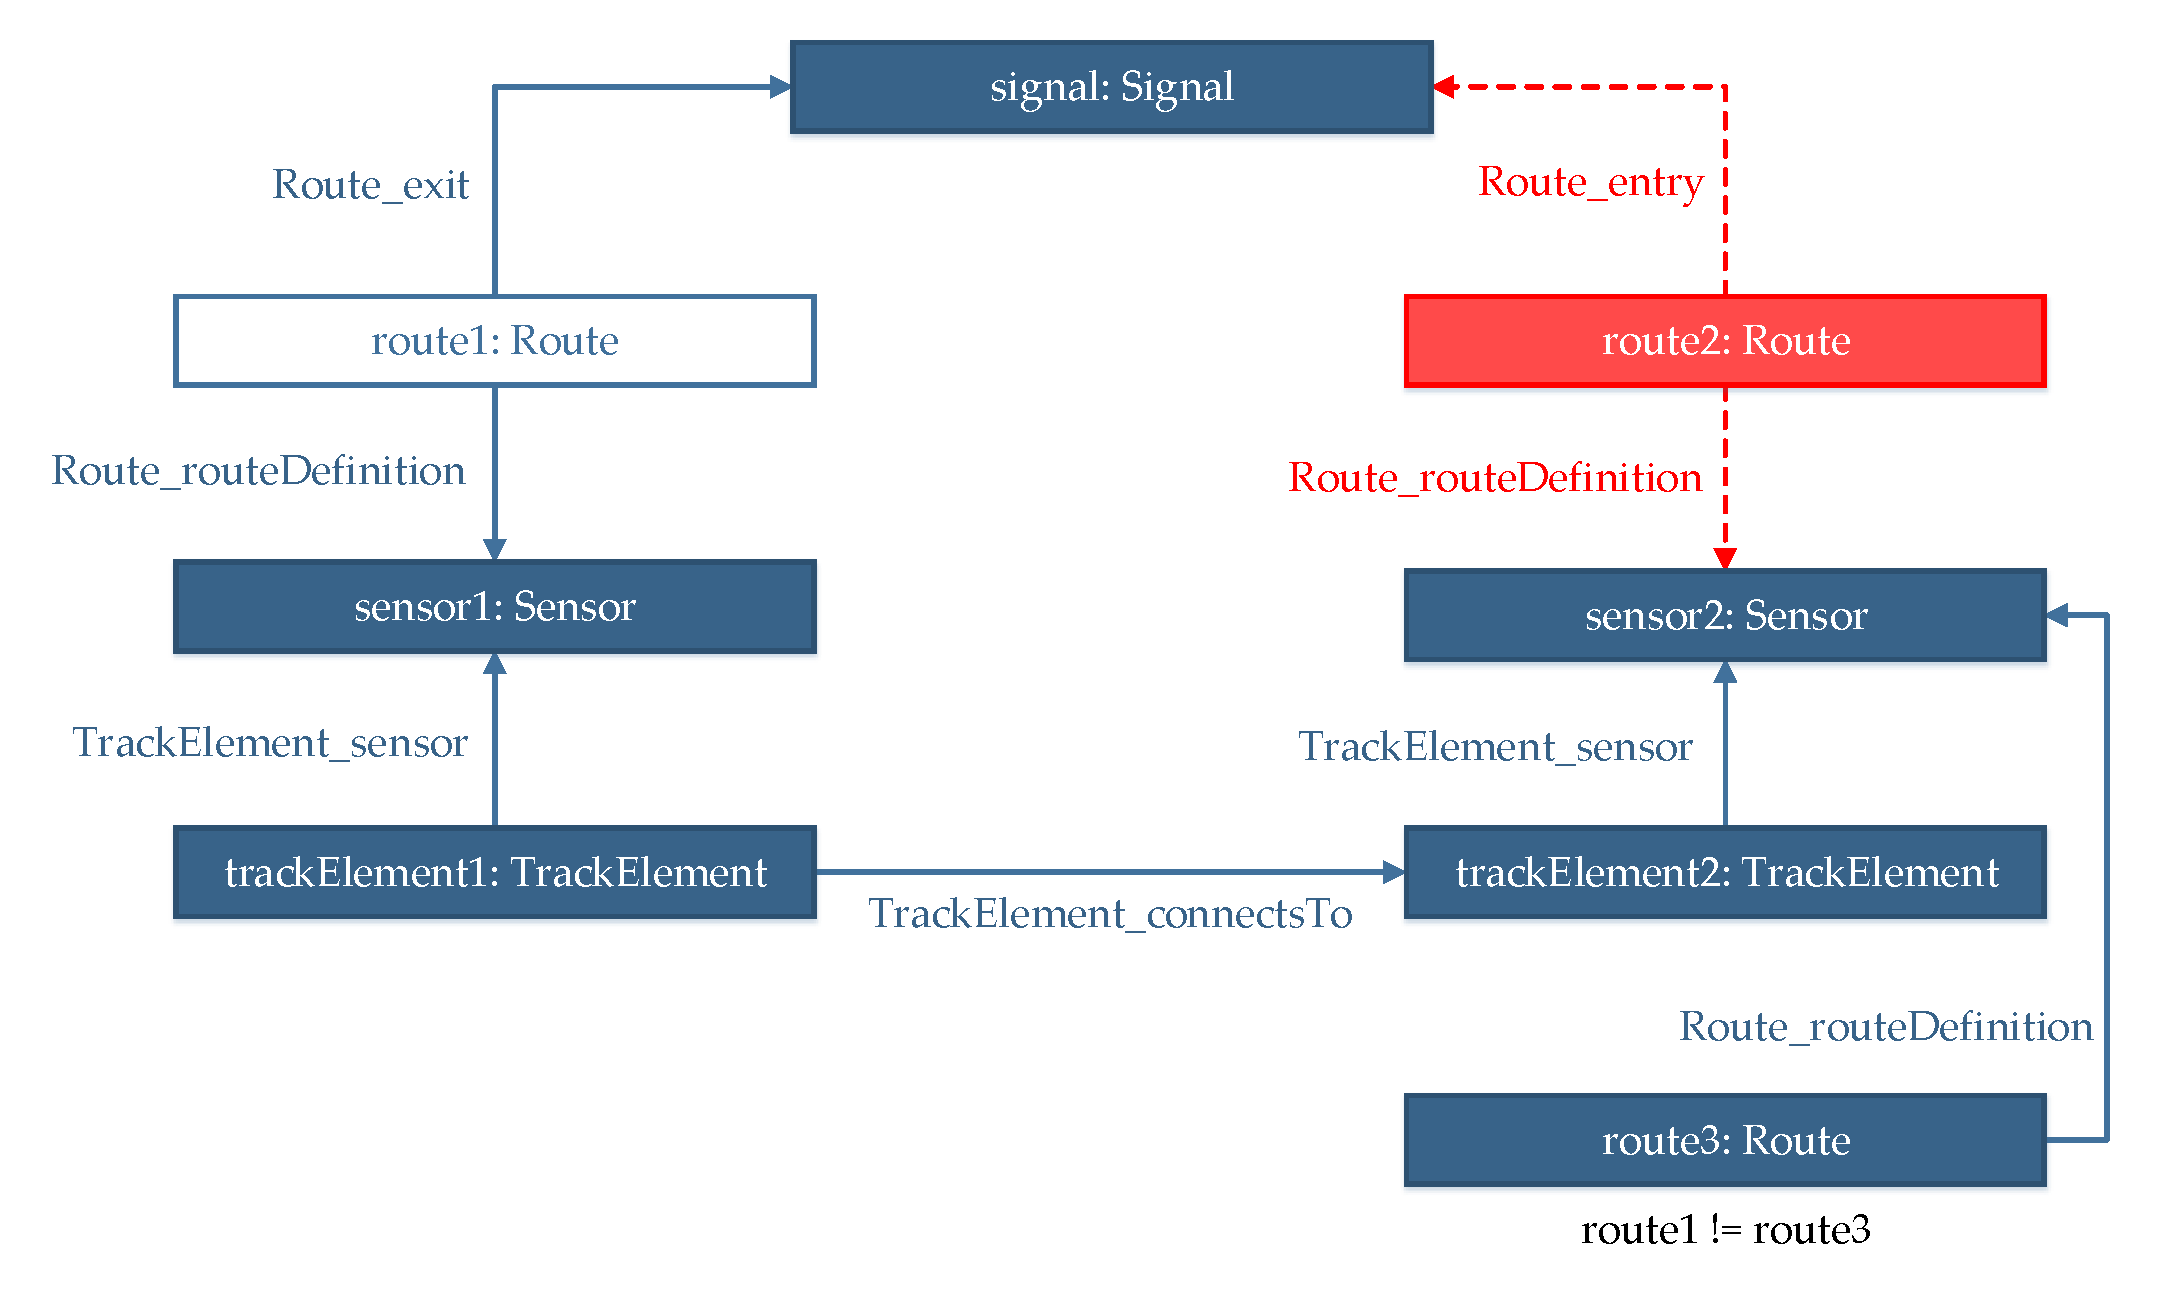
\includegraphics[scale=0.4]{figures/trainbenchmark-signalneighbor}
		\caption{The SignalNeighbor query's pattern}
		\label{fig:trainbenchmark-signalneighbor}
\end{figure}

\paragraph{Relational algebraic form.} The \textit{SignalNeighbor} query can be formalized in relational algebra as:

\begin{align*}
& \pi_{\mathit{Route\_entry.Route}} \big( \sigma_{\mathit{Route\_entry.Route} \neq \mathit{Route\_routeDefinition_2.Route}} \big( \\
& \quad \mathit{Route\_entry} \naturaljoin \mathit{Route\_routeDefinition_1} \naturaljoin \mathit{TrackElement\_sensor_1} \naturaljoin \\
& \quad \mathit{TrackElement\_connectsTo} \naturaljoin \mathit{TrackElement\_sensor_2} \naturaljoin \mathit{Route\_routeDefinition_2} \antijoin \\
& \quad \left( \mathit{Route\_exit} \naturaljoin \mathit{Route\_routeDefinition_3} \right) \\
& \big) \big)
\end{align*}

%%%%%%%%%%%%%%%%%%%%%%%%%%%%%%%%%%%%%%%%%%%%%%%%%%%%%%%%%%%%%%%%%%%%%%%%%%%%%%%
\subsubsection{SwitchSensor}

\paragraph{Description.} The \textit{SwitchSensor} well-formedness constraint requires that every switch must have at least one sensor connected to it. Therefore, the query (\figref{fig:trainbenchmark-switchsensor}) checks for switches that have no sensors associated with them. The SPARQL representation of the query is shown in \lstref{lst:switchsensor-sparql}.

\paragraph{Goal.} This query checks whether an object is connected to a relation. This pattern is common in more complex queries, e.g.\ it is used the \textit{RouteSensor} and the \textit{SignalNeighbor} queries.

\begin{figure}[Htb]
\centering
\begin{minipage}{0.5\textwidth}
  { \alignListing
    \sourceSPARQL{figures/queries/SwitchSensor_neg.sparql}}
  \caption{SwitchSensor query in SPARQL}
  \label{lst:switchsensor-sparql}
\end{minipage}
\end{figure}

% \begin{lstlisting}[caption=The RouteSensor query in SPARQL, label=lst:switchsensor-sparql]
% PREFIX base: <http://www.semanticweb.org/ontologies/2011/1/TrainRequirementOntology.owl#>
% PREFIX rdfs: <http://www.w3.org/2000/01/rdf-schema#>
% PREFIX owl:  <http://www.w3.org/2002/07/owl#>
% PREFIX rdf:  <http://www.w3.org/1999/02/22-rdf-syntax-ns#>
% 
% SELECT DISTINCT ?xSwitch
% WHERE
% {
%   ?xSwitch rdf:type base:Switch .
% 
%   OPTIONAL { 
%            ?xSensor rdf:type base:Sensor .
%            ?xSwitch base:TrackElement_sensor ?xSensor .
%            } .
%   FILTER (!BOUND(?xSensor))
% }
% \end{lstlisting}


\begin{figure}[Htb]
		\centering
		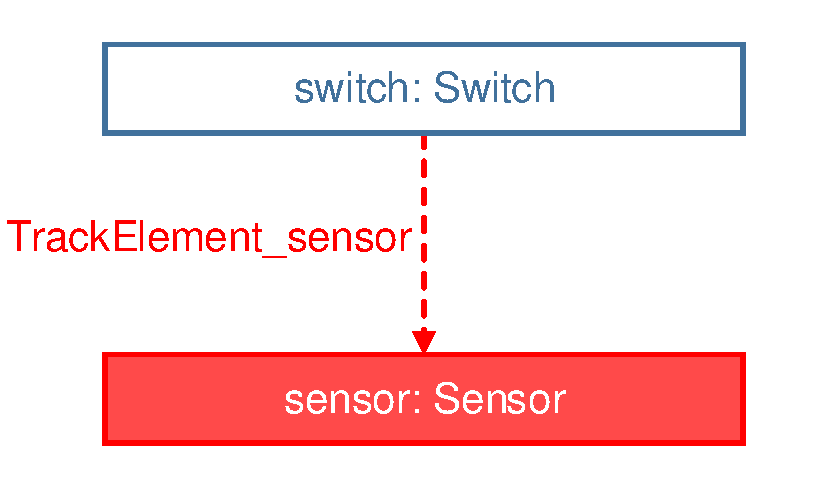
\includegraphics[scale=0.4]{figures/trainbenchmark-switchsensor}
		\caption{The SwitchSensor query's pattern}
		\label{fig:trainbenchmark-switchsensor}
\end{figure}

\paragraph{Relational algebraic form.} The \textit{SwitchSensor} query can be formalized in relational algebra as:

$$ \mathit{Switch} \antijoin \mathit{Sensor} $$


\subsection{Transformations}
\label{sec:transformatios}

In the \emph{edit} phase the model is modified to change the result set returned in the succeeding re-check phase.

\todo{táblázat grafikai megjelenésén javítani}

\begin{table}[Htb]
	\centering
	\scriptsize
	\begin{tabular}{r|r|r|r|r|r|r|r|r|r|}
	\cline{2-9}
	& \multicolumn{4}{ c| }{\bf User (modify = 10)} & \multicolumn{4}{ c| }{\bf Model transformation (modify = Res1 × 10\%)} \\ \hline
	\multicolumn{1}{ |r| }{\bf\#Objects} & \bf \#Sensors & \bf Result1 & \bf Modify RS & \bf Result2 & \bf \#Sensors & \bf Result1 & \bf Modify RS & \bf Result2 \\ \hline
	\multicolumn{1}{ |r| }{6032}         & 928 & 19 & 10 & 29 & 967 & 94 & 9 & 85 \\ \hline
	\multicolumn{1}{ |r| }{11710}        & 1804 & 41 & 10 & 51 & 1936 & 193 & 19 & 174 \\ \hline
	\multicolumn{1}{ |r| }{23180}        & 3575 & 68 & 10 & 76 & 3545 & 348 & 34 & 314 \\ \hline
	\multicolumn{1}{ |r| }{46728}        & 7210 & 140 & 10 & 150 & 6691 & 642 & 64 & 578 \\ \hline
	\multicolumn{1}{ |r| }{87396}        & 13465 & 264 & 10 & 274 & 13650 & 1301 & 130 & 1171 \\ \hline
	\multicolumn{1}{ |r| }{175754}       & 27074 & 510 & 10 & 520 & 27190 & 2606 & 260 & 2346 \\ \hline
	\multicolumn{1}{ |r| }{354762}       & 54653 & 1048 & 10 & 1058 & 55708 & 5324 & 532 & 4792 \\ \hline
	\multicolumn{1}{ |r| }{708770}       & 109185 & 2071 & 10 & 2081 & 110291 & 10623 & 1062 & 9561 \\ \hline
	\multicolumn{1}{ |r| }{1415954}      & 218140 & 4215 & 10 & 4224 & 219305 & 21097 & 2109 & 18988 \\ \hline
	\multicolumn{1}{ |r| }{2837336}      & 437089 & 8501 & 10 & 8510 & 437025 & 41762 & 4176 & 37586 \\ \hline
	\end{tabular}
\caption{Modification in the RouteSensor test case}
\label{tbl:modify_RouteSensor}
\end{table}

\autoref{tbl:modify_RouteSensor}. shows instance model characteristics and the effect of the modify phase in the \emph{RouteSensor} case. The first column counts the number of instance model elements, and the second shows the number of Sensors, which can be erroneous. The two scenarios process different instance models, and modifies them differently:

\begin{itemize}
\item 
In the \emph{User scenario} (where a developer is assumed to sit in front of an editor) the initial number of constraint violating elements are low (0.3\% of model elements for the RouteSensor case), so it can be understood and resolved by a human using the editor.

During the modification the user always performs ten random edits (fixed low constant) which increase the number of erroneous elements. These edit operations modify only some elements of the model, and does not add or remove modules containing multiple instance model elements.

\item 
In the \emph{model transformation scenario} the initial number of errors is higher (1.5\% of objects for the RouteSensor case). This scenario models the case when these errors are processed by a model transformation program automatically.

In the edit phase the program modifies ten percent of the elements of the result set originating from the batch query. These modifications always correct the model, thus the number of invalid elements decreases (see \autoref{tbl:modify_type}).

\end{itemize}


\autoref{tbl:modify_type}. displays the effect of model changes to the result set size, and the type of edit operations (add, update, delete).

\begin{table}[h]
	\centering
	\begin{tabular}{l|l|l|l|l|l|}
	\cline{2-5}
	& \multicolumn{2}{ c| }{\bf User} & \multicolumn{2}{ c| }{\bf Model transformation} \\ \cline{2-5}
	& \bf Modification type & \bf RSS change & \bf Modification type & \bf RSS change \\ \hline
	\multicolumn{1}{ |l| }{\bf PosLength}      & Update & Increase & Update & Decrease \\ \hline
	\multicolumn{1}{ |l| }{\bf SwitchSensor}   & Delete & Increase & Add    & Decrease \\ \hline
	\multicolumn{1}{ |l| }{\bf RouteSensor}    & Delete & Increase & Delete & Decrease \\ \hline
	\multicolumn{1}{ |l| }{\bf SignalNeighbor} & Update & Increase & Update & Decrease \\ \hline
	\end{tabular}
	\caption{Modification type for the queries}
	\label{tbl:modify_type}
\end{table}

\begin{figure}[!Htb]
	\centering
	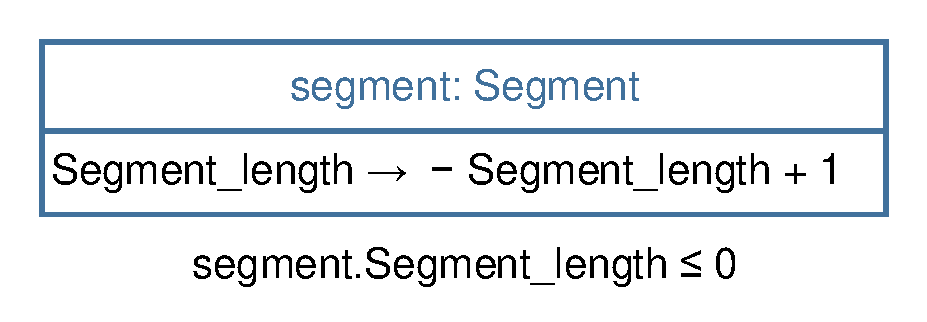
\includegraphics[scale=0.4]{figures/trainbenchmark-transformation-xform-poslength}
	\caption{The PosLength query's transformation in the Model transformation scenario}
	\label{fig:trainbenchmark-transformation-xform-poslength}
\end{figure}

\begin{figure}[!Htb]
	\centering
	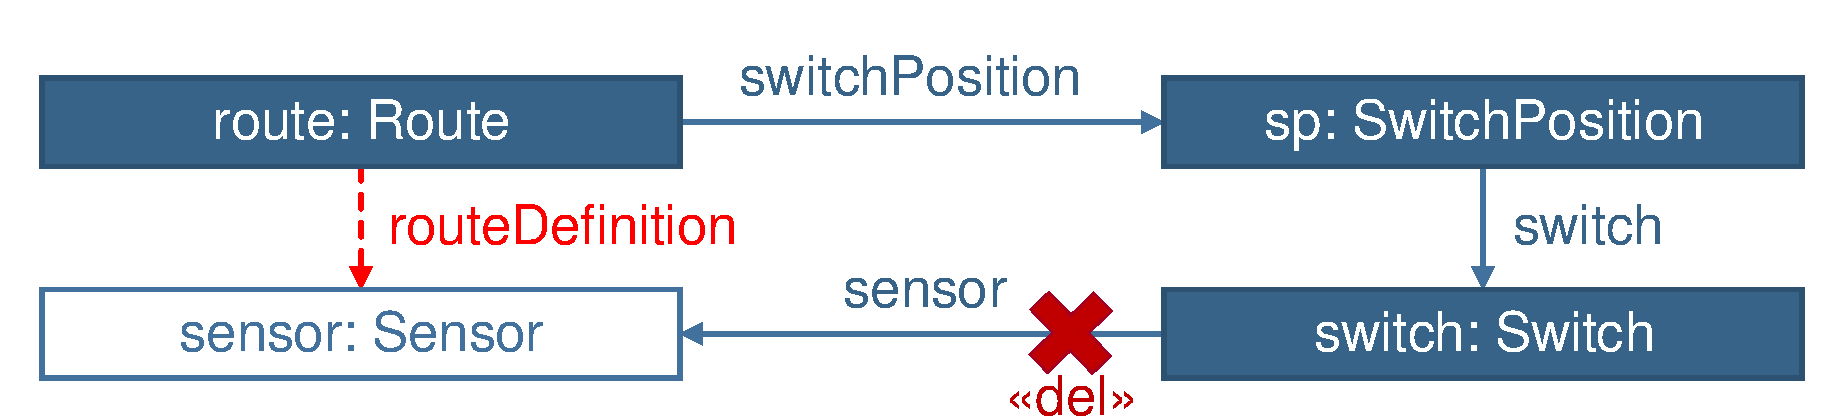
\includegraphics[scale=0.4]{figures/trainbenchmark-transformation-xform-routesensor}
	\caption{The RouteSensor query's transformation in the Model transformation scenario}
	\label{fig:trainbenchmark-transformation-xform-routesensor}
\end{figure}

\begin{figure}[!Htb]
	\centering
	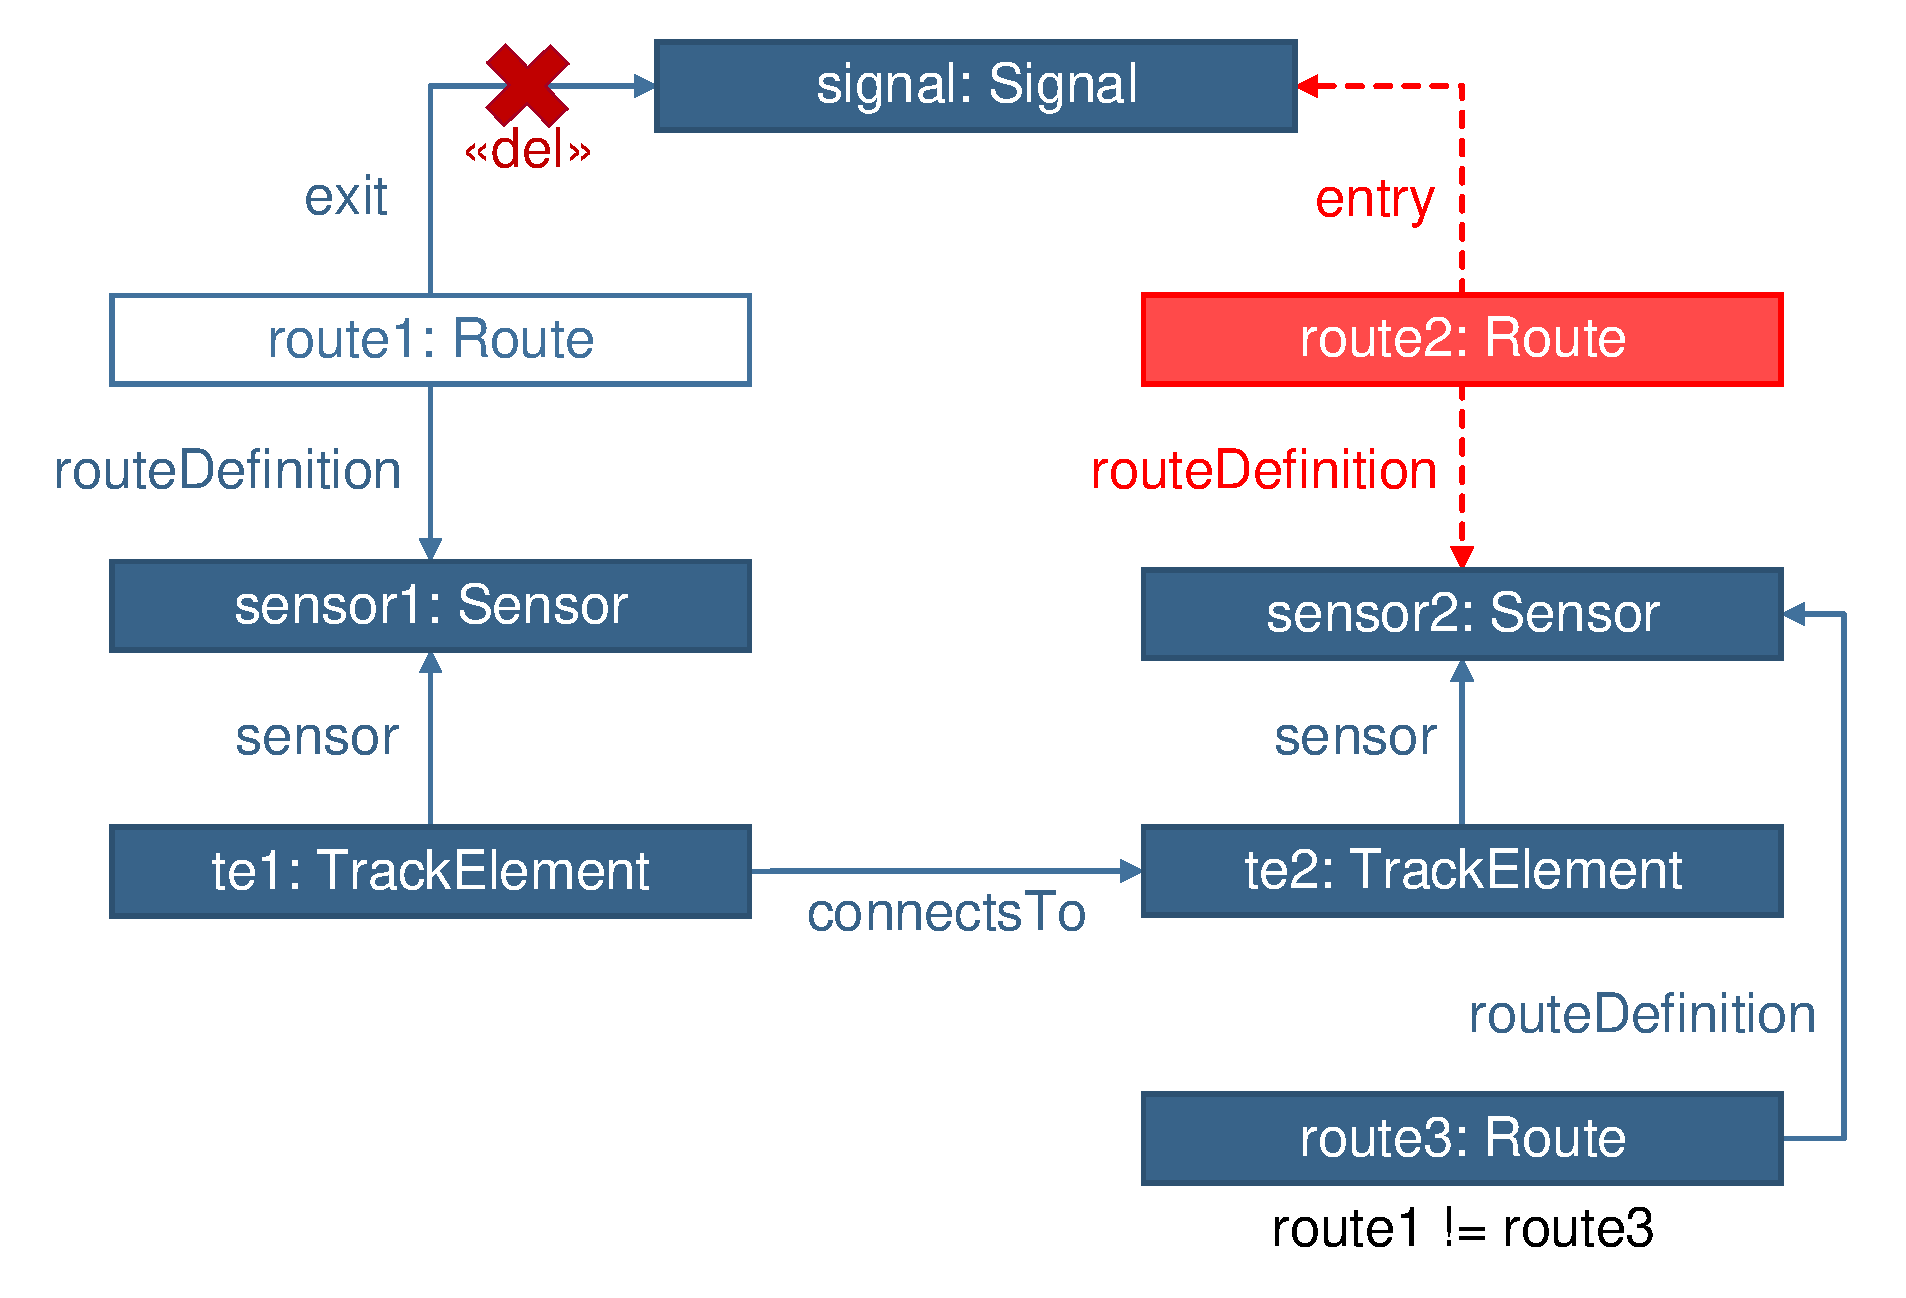
\includegraphics[scale=0.4]{figures/trainbenchmark-transformation-xform-signalneighbor}
	\caption{The SignalNeighbor query's transformation in the Model transformation scenario}
	\label{fig:trainbenchmark-transformation-xform-signalneighbor}
\end{figure}

\begin{figure}[!Htb]
	\centering
	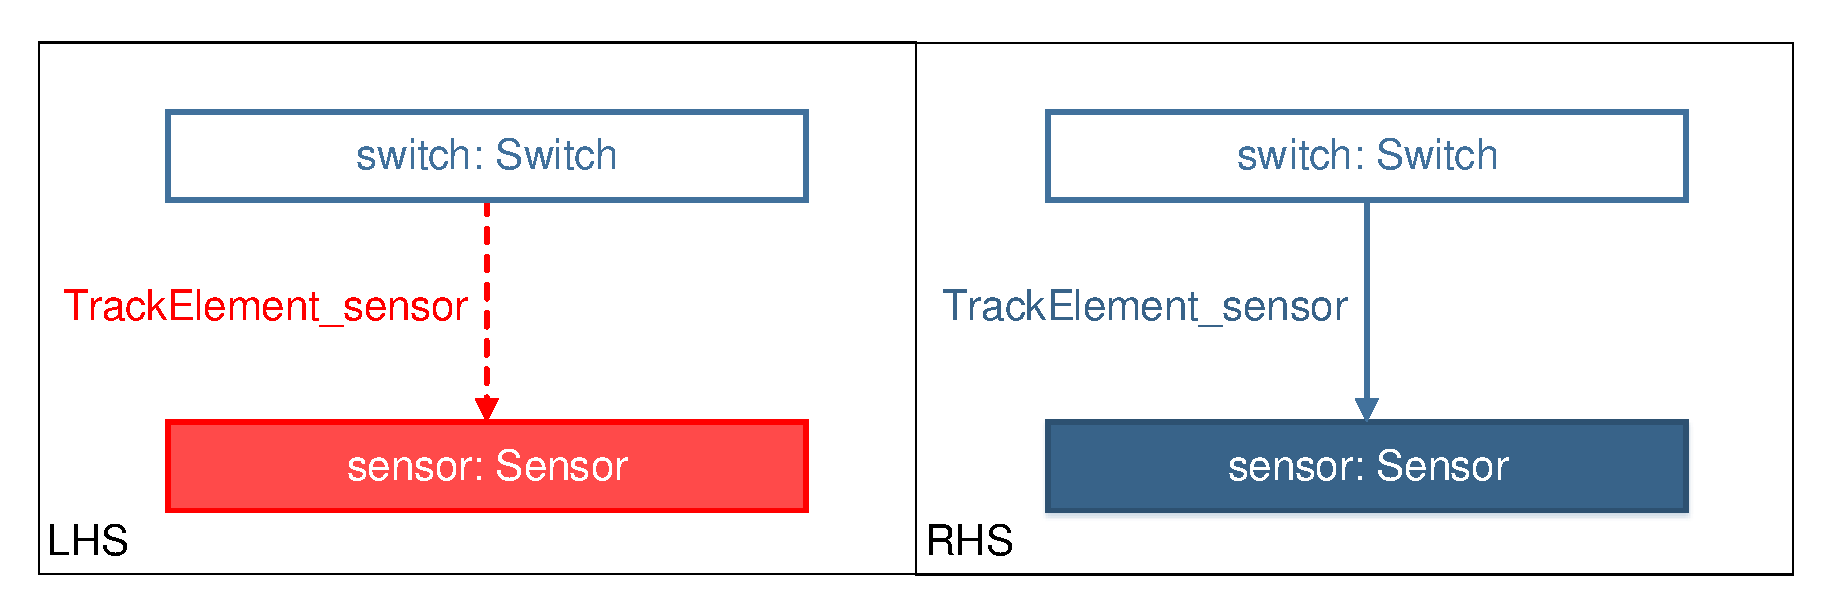
\includegraphics[scale=0.4]{figures/trainbenchmark-transformation-xform-switchsensor}
	\caption{The SwitchSensor query's transformation in the Model transformation scenario}
	\label{fig:trainbenchmark-transformation-xform-switchsensor}
\end{figure}



\begin{figure}
        \centering
        \begin{subfigure}[b]{0.25\textwidth}
                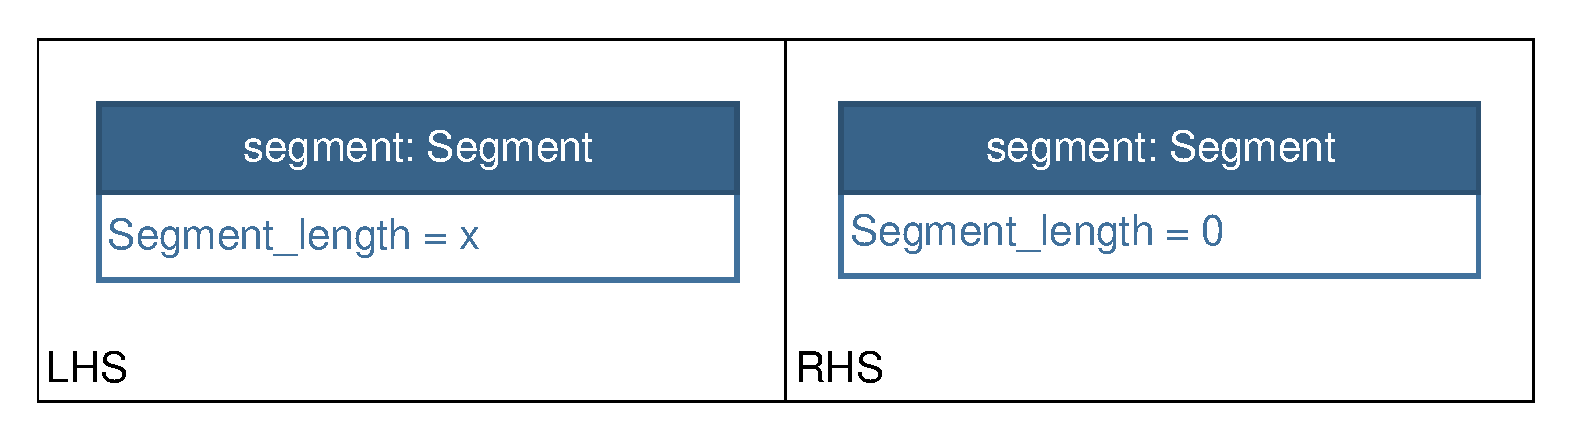
\includegraphics[width=\textwidth]{figures/trainbenchmark-transformation-user-poslength}
                \caption{PosLength}
                \label{fig:trainbenchmark-transformation-user-poslength}
        \end{subfigure}
        ~
        \begin{subfigure}[b]{0.3\textwidth}
                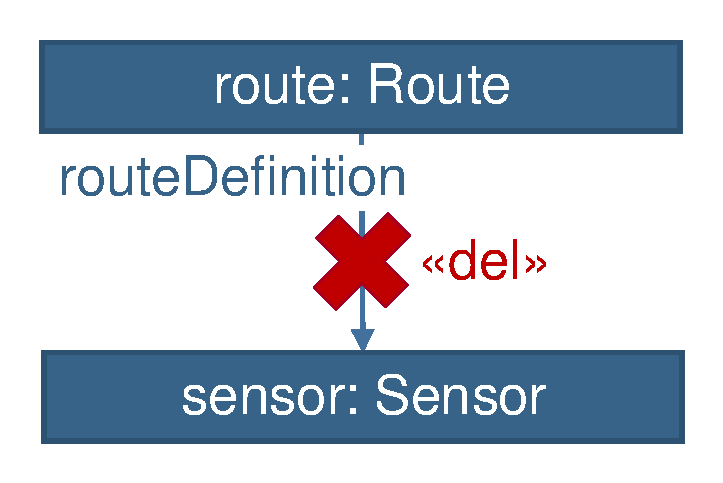
\includegraphics[width=\textwidth]{figures/trainbenchmark-transformation-user-routesensor}
                \caption{RouteSensor}
                \label{fig:trainbenchmark-transformation-user-routesensor}
        \end{subfigure}%
        ~
        \begin{subfigure}[b]{0.3\textwidth}
                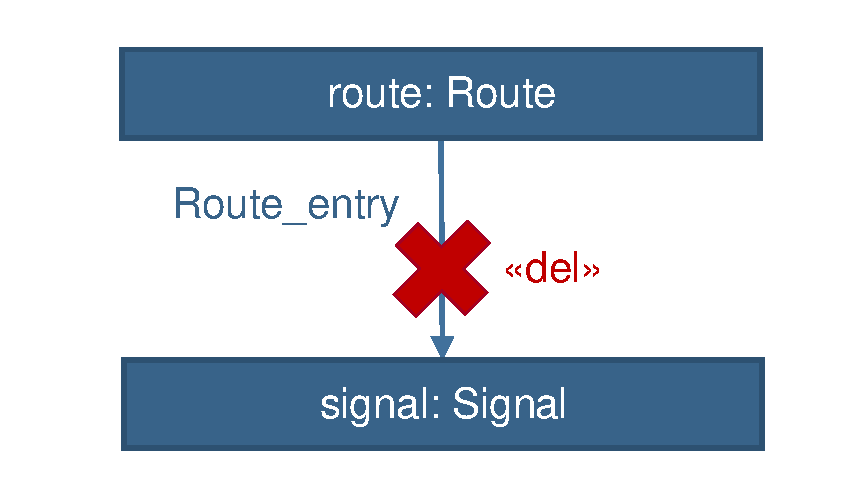
\includegraphics[width=\textwidth]{figures/trainbenchmark-transformation-user-signalneighbor}
                \caption{SignalNeighbor}
                \label{fig:trainbenchmark-transformation-user-signalneighbor}
        \end{subfigure}%
        ~
        \begin{subfigure}[b]{0.3\textwidth}
                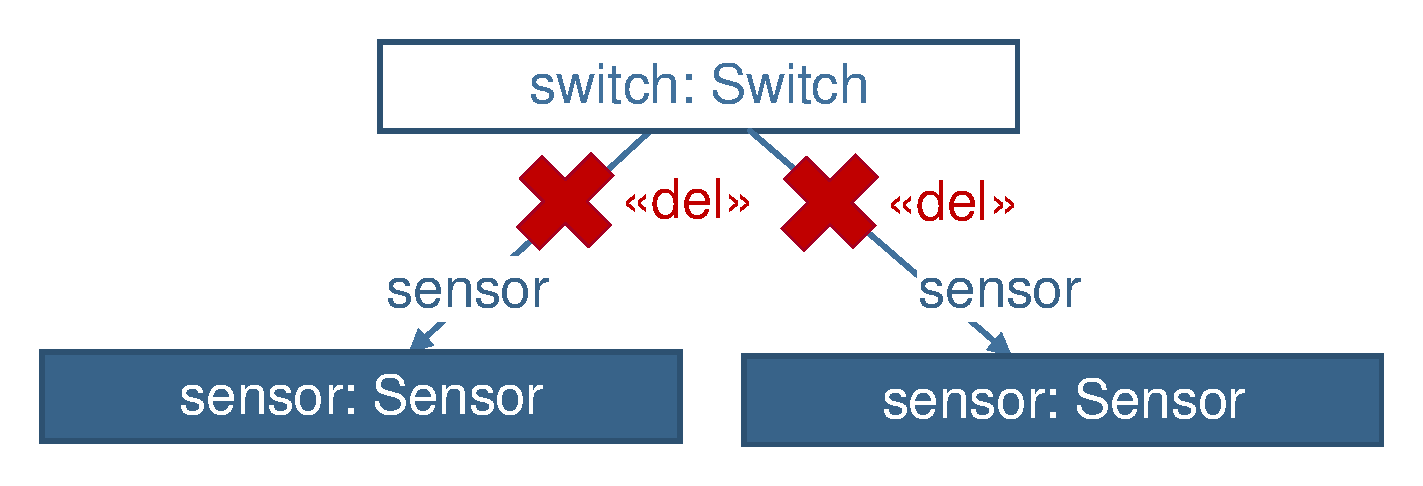
\includegraphics[width=\textwidth]{figures/trainbenchmark-transformation-user-switchsensor}
                \caption{SwitchSensor}
                \label{fig:trainbenchmark-transformation-user-switchsensor}
        \end{subfigure}
        \caption{Transformations in the User scenario}\label{fig:animals}
\end{figure}


The modifications in more detail:
\begin{itemize}
  \item \emph{User scenario:} in this case elements to be edited are selected from the whole instance model, i.e. they may be valid or invalid. 
  \begin{itemize}
    
    \item \emph{PosLength:} In this query's modify phase a randomly selected segment's length is updated to 0, which means that an error is injected \figref{fig:trainbenchmark-transformation-user-poslength}.
    
    In EMF this means that an int attribute is set (updated), while in other graph databases (e.g. RDF databases) first the assertions about the old value is removed, and the assertion stating the new value of the length is inserted.
    
    \item \emph{RouteSensor:} The route definition connection between the randomly selected routes' and their first connected sensor are removed \figref{fig:trainbenchmark-transformation-user-routesensor}.
    
    \item \emph{SignalNeighbor:} Errors are introduced by unconnecting the entry edge of the selected routes \figref{fig:trainbenchmark-transformation-user-signalneighbor}.

    \item \emph{SwitchSensor:} Errors are injected by randomly selecting switches and deleting their relationship to sensors. If the chosen switch was invalid, it stays invalid (as no relationships are deleted); if the chosen switch was valid, it will become invalid \figref{fig:trainbenchmark-transformation-user-switchsensor}.
        
  \end{itemize}
  \item \emph{Model transformation scenario:} in this case elements to be edited are selected from the result of the previous query.
  \begin{itemize}
    
    \item \emph{PosLength:} Random elements selected from the set of invalid elements, and their values are negated: updated to $-1 \times (\mathit{oldValue}-1)$ \figref{fig:trainbenchmark-transformation-xform-poslength}.
    
    \item \emph{RouteSensor:} The erroneous sensors are removed from the switch, which means that the constaint must no longer apply \figref{fig:trainbenchmark-transformation-xform-routesensor}.
    
    \item  \emph{SignalNeighbor:} Disconnect \emph{exit} references of erroneous routes, resulting in a structure where the constraint must not be hold for the actual route \figref{fig:trainbenchmark-transformation-xform-signalneighbor}.
    
    \item \emph{SwitchSensor:} For selected invalid switches sensors are created, and connected to them.
    In EMF this means the creation of a new Sensor, and it is added to the switch, and also to the root container object. In ontology the triples asserting the connection between the new Sensor and the switch, as well as its type are inserted into the knowledge base \figref{fig:trainbenchmark-transformation-xform-switchsensor}.  
    
  \end{itemize}
\end{itemize}
 


\subsection{Instance Model Generation}
\label{sec:instanceGeneration}

In the first phase of the benchmark, a previously generated \concept{instance model} is loaded from the file system. These models are systematically generated based on the metamodel and on the model queries. Randomized instance model fragments are generated and connected to each other. The generation process takes care of controlling the number of matches for all model queries.

To break symmetry, the exact number of elements and cardinalities are randomized. This brings artificially generated models \emph{closer to real world instances}, and \emph{prevents query tools from this kind of efficient storing} of instance models. During the generation of the railway system model, errors are injected at random positions. The initial number of constraint violating elements that are low (below one percent of the total number of elements), and are deterministically placed, thanks to \emph{pseudo} random generation. These errors have to be found in the check phase of the benchmark, and can be corrected during the edit phase.

\begin{figure}[Htb]
\begin{center}
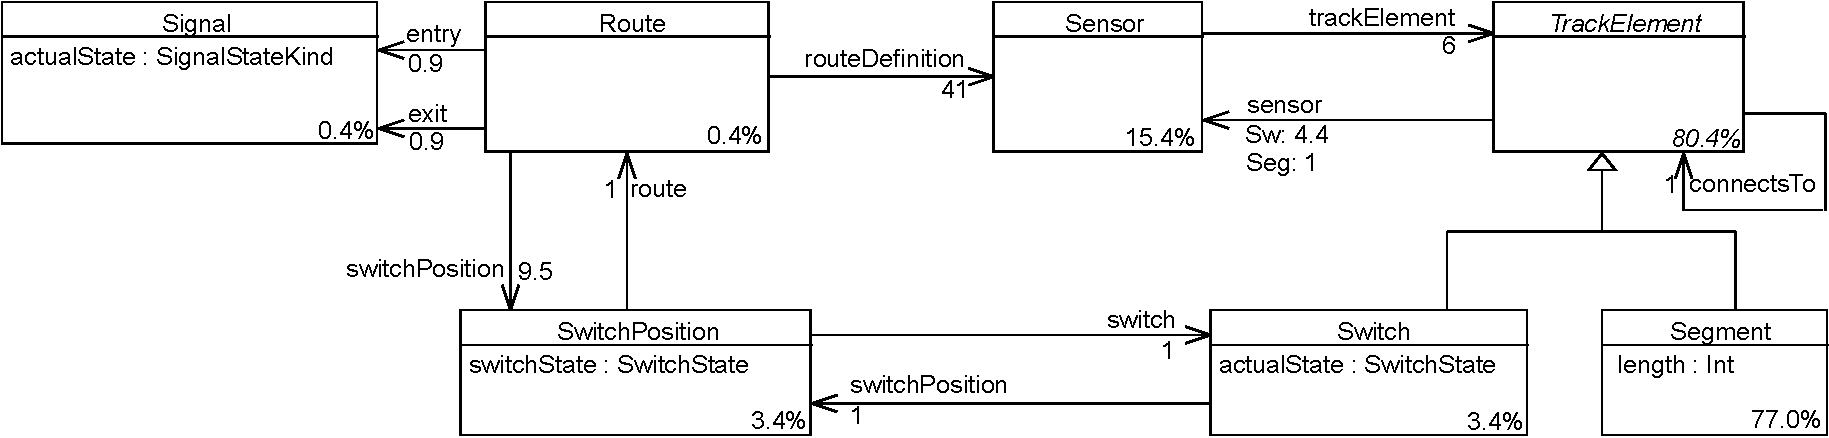
\includegraphics[width=0.9\textwidth]{figures/instance/TrainMMb.pdf}
\caption{Train Metamodel and Instance Model Characteristics}
\label{fig:metamodel-instance-characteristics}
\end{center}
\end{figure}

To show some characteristics of the generated instance models, the distribution of the object types and the average number of edges for each object are presented in \autoref{fig:metamodel}. In the case of classes the percentage of instances is shown: e.g., 3.4\% of the model elements are instance of the class \emph{Switch}, 77.0\% is \emph{Segment}, thus 80.4\% of the model is TrackElement. The average number of the given relation for an instance is displayed for associations: e.g., there are 9.5 \emph{switchPosition} relations in average for every instance of the \emph{Route} class.